At the end of this worksheet you should be able to  
\begin{itemize}
	\item calculate the new quantities of pressure, gauge pressure, and density.
	\item apply the new principles of Pascal, Archimedes, and Bernoulli.  
	\item use the continuity principle to solve for an unknown quantity.
	\item use the hydrostatic pressure principle to solve for an unknown quantity.
\end{itemize}

You will want to keep the following table of densities from your textbook handy.

\centering
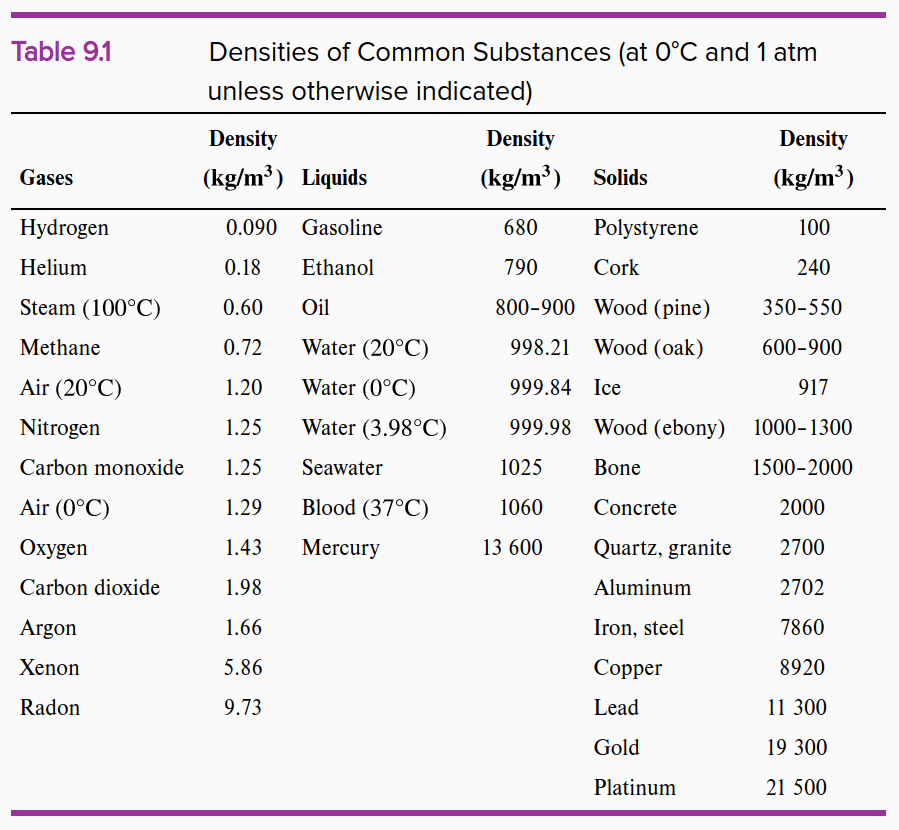
\includegraphics[scale=.35]{week11-figures-density.png}

\begin{enumerate}
	\setlength\itemsep{2 in}
	
	\item If \SI{500}{N} person stands on one foot that has an area \SI{50.0}{cm^2}, what is the pressure on the floor? If this person stands on their heel in a high heeled shoe that has an area of \SI{1.00}{cm^2}, what pressure is there? What if this person stands on a diamond that is cut to have a bottom facet that is \SI{10000}{\micro\meter^2} ($\SI{1}{\micro\meter}=\SI{e-6}{\meter}$)? \emph{(Careful with unit conversions!)}.
	
	\item
	A patient's blood systolic blood pressure when resting is 160 mmHg. What is this pressure in pascals, psi, and atm?
	
	\item
	Throughout this worksheet and the homework \emph{gauge pressure} is a way of expressing the pressure measured by an instrument relative to the atmospheric pressure. So \SI{1}{atm} of absolute pressure is set to \SI{0}{atm} of gauge pressure. Perfect vacuum is absolute zero pressure, so that would be \SI{-1}{atm} of gauge pressure. So what is \SI{2}{atm} of gauge pressure as atmospheric pressure? \SI{30}{\kilo\pascal} of absolute pressure is what gauge pressure? What about a gauge pressure of \SI{1000}{\kilo\pascal} as absolute pressure?
	
	\item
	In a hydraulic lift, the radius of a small piston is \SI{2}{cm} and the radius of the larger piston is \SI{20}{cm}, what weight can the larger piston support when a force of \SI{250}{N} is applied to the smaller piston? If the larger piston moves \SI{5}{cm}, how far does the small piston move?\bigskip
	
	\item
	At the surface of a freshwater lake, the air pressure is \SI{1}{atm}. At what depth under the water is the absolute pressure \SI{4}{atm}? \bigskip
	
	\item 
	At sea level, the average atmospheric pressure is \SI{1}{atm}. The density of air at this level is about \SI{1.29}{kg/m^3}. Assuming the density of air is constant (its not but just go with it), what is the air pressure at the Empire State Building that has a height of \SI{381}{\meter} at the top deck, and we will just assume that its base is at sea level?
	
	\item 
	A diver swims to a depth of 10 meters in a lake. What is the pressure on the diver's body? What is the force on the diver's eardrums from the water if the area of the eardrum is \SI{0.60}{cm^2}? What would this be if the diver was swimming in sea water? (Ignore the fact that there is atmospheric pressure inside the eardrum, but also think about this problem if you didn't ignore that fact.)
	
	\item
	A \SI{5000}{\newton} object is floating in fresh water. 
	\begin{itemize}
		\setlength\itemsep{1 in}
		\item What is the net force on the object?
		\item What is the magnitude of the buoyant force?
		\item If the the bottom of the object is \SI{1}{meter} below the surface of the water, then what pressure is on the bottom of the object?
		\item What is the area of the bottom surface of the object?
		\item If the object has another \SI{1}{\meter} sticking out of the water, then what is the volume of the object?
		\item What is its density?	
	\end{itemize}
	
	\item
	The following cylindrical barrels are filled to the brim with fluids of the given density. Put these in order from smallest to largest pressure at the bottom of the barrel.
	\begin{enumerate}
		\item $R=\SI{40}{cm}, h=\SI{80}{cm}, \rho=\SI{1000}{kg/m^3}$
		\item $R=\SI{40}{cm}, h=\SI{100}{cm}, \rho=\SI{1000}{kg/m^3}$
		\item $R=\SI{50}{cm}, h=\SI{100}{cm}, \rho=\SI{800}{kg/m^3}$
		\item $R=\SI{50}{cm}, h=\SI{80}{cm}, \rho=\SI{800}{kg/m^3}$
		\item $R=\SI{50}{cm}, h=\SI{125}{cm}, \rho=\SI{800}{kg/m^3}$
	\end{enumerate}\bigskip
	
	
	\item 
	Let's do a problem based on the famous Archimedes legend. The story goes that a King Hiero II of Syracuse commissioned an ornate golden crown to be made, but when he got it, he was suspicious that silver had been mixed in with the gold. He charged Archimedes to figure out how to determine the density of the crown without damaging it. Archimedes' ``Eureka'' moment came when he realized he could determine the volume of a complex shape by submerging it in a tub of water that had been filled to the brim. The amount of water that spilled over the edge would be equal to the volume of the crown as long as you could catch all of the spilled water and measure its volume. So with all of that said, suppose the amount of water that spilled over the edge weighed \SI{1.0}{\newton} but there was still some water stuck to the sides of the bucket that didn't get weighed so maybe call it \SI{1.1}{\newton} I don't know this is pretty messy. The crown itself weighed \SI{24.1}{\newton}. So what is the density of the crown and how does it compare to gold? \emph{Hint: what is the volume of water that spilled over the edge?}
	
	\item
	The above story is ridiculous. What if the water that spilled over the edge had weighed \SI{1.2}{\newton} or \SI{1.0}{\newton}? This is far too imprecise for something as serious as an allegation of cheating the king out of a pure gold crown. So instead we want to measure the buoyant force on the crown. So, if you weight the crown to be \SI{24.1}{\newton} and then you lower it into the water fully submerged and weight it then (by tying a string to it and lowering it into the water but the string is attached to a balance) and then its ``weight'' is \SI{22.85}{\newton}. What is the buoyant force upward on the crown? What volume of water has been displaced? What is the volume of the crown? What is the density of the crown? What is better about this method?
	\bigskip
	
	\item
	``ICEBERG DEAD AHEAD!'' It is sometimes said that only 10\% of an iceberg's volume actually sticks out above the surface of the water which is what made it so deadly to poor Jack and Rose on the \emph{Titanic}. If the density of ice is \SI{917}{\kg/m^3} and the density of seawater is \SI{1025}{kg/m^3}, then what is the ratio of the volume of ice under the water to the entire volume of ice? What is the ratio of the volume of ice above the water to the entire volume of ice?  Next work these \emph{in general} for any density of object floating in any density of fluid. 
	
	\item
	An artery has an inner diameter of 1.5 mm, but narrows to an inner diameter of 1.0 mm due to a build up of plaque. By what percent does the speed of blood flow change when it enters the narrow section?
	
	\item 
	What if we have a case where a single pipe splits into many pipes. Following an example from the textbook, the aorta is the artery from your heart that feeds 32 other major arteries. The aorta has an inner radius of \SI{1}{cm} and assume each of the other arteries has an inner radius of \SI{0.21}{cm}. If blood in the aorta has an average speed of \SI{28}{cm/s}, then what is the average speed of blood in the major arteries? \emph{Hint: you can just treat the major arteries as one big pipe that has an area 32 times bigger than the area of a single artery.}
	
	\item
	Suppose it takes one minute to fill a 5 gallon bucket with water from your garden hose that is open all the way. The diameter of your hose is \SI{1}{inch}. How fast is water traveling out of the end of the hose? How fast does it travel if you hold your thumb over the end of the hose and cover half of the area of the hose? (\SI{1}{inch}=\SI{0.0254}{m}, \SI{1}{gallon}=\SI{0.00378}{m^3}, \SI{1}{min}=\SI{60}{s})
	
	\item
	Show that Bernoulli's Principle really just reduces to the equation for pressure as a result of gravity when the fluid is not flowing (so $v_1=v_2=0$). This equation is now the same as the \emph{hydrostatic pressure} equation. 
	
	\item
	A cylindrical container of water is full to the brim when a hole is punctured \SI{0.5}{\meter} from the top. What is the speed of the water as it comes out of the hole?
	
	\item 
	Following up on the previous problem, if you redirected this water straight up with the same speed, how high would it rise?
	
	\item
	If water flows horizontally through a hose that has a radius of \SI{1}{cm} at a speed of \SI{2}{m/s}. If the nozzle of the hose narrows to \SI{0.25}{cm} as the water sprays out, then what is the pressure inside the hose? What is it as a gauge pressure?
	
	
\end{enumerate}